\appendix
%% Правка оформления ссылок на приложения:
%http://tex.stackexchange.com/questions/56839/chaptername-is-used-even-for-appendix-chapters-in-toc
%http://tex.stackexchange.com/questions/59349/table-of-contents-with-chapter-and-appendix
%% требует двойной компиляции
\addtocontents{toc}{\def\protect\cftchappresnum{\appendixname{} }%
\setlength{\cftchapnumwidth}{\widthof{\cftchapfont\appendixname~Ш\cftchapaftersnum}}%
}
%% Оформление заголовков приложений ближе к ГОСТ:
\sectionformat{\chapter}[display]{% Параметры заголовков разделов в тексте
    label=\chaptertitlename\ \thechapter,% (ГОСТ Р 2.105, 4.3.6)
    labelsep=20pt,
}
\renewcommand\thechapter{\Asbuk{chapter}} % Чтобы приложения русскими буквами нумеровались

%\chapter{Программный код алгоритма идентификации на основе расходно-напорных характеристик имплантируемого роторного насоса крови HeartMate II}

\chapter{Акты о внедрении результатов диссертационной работы} \label{AppendixC}

\begin{figure}[ht] 
  \center
  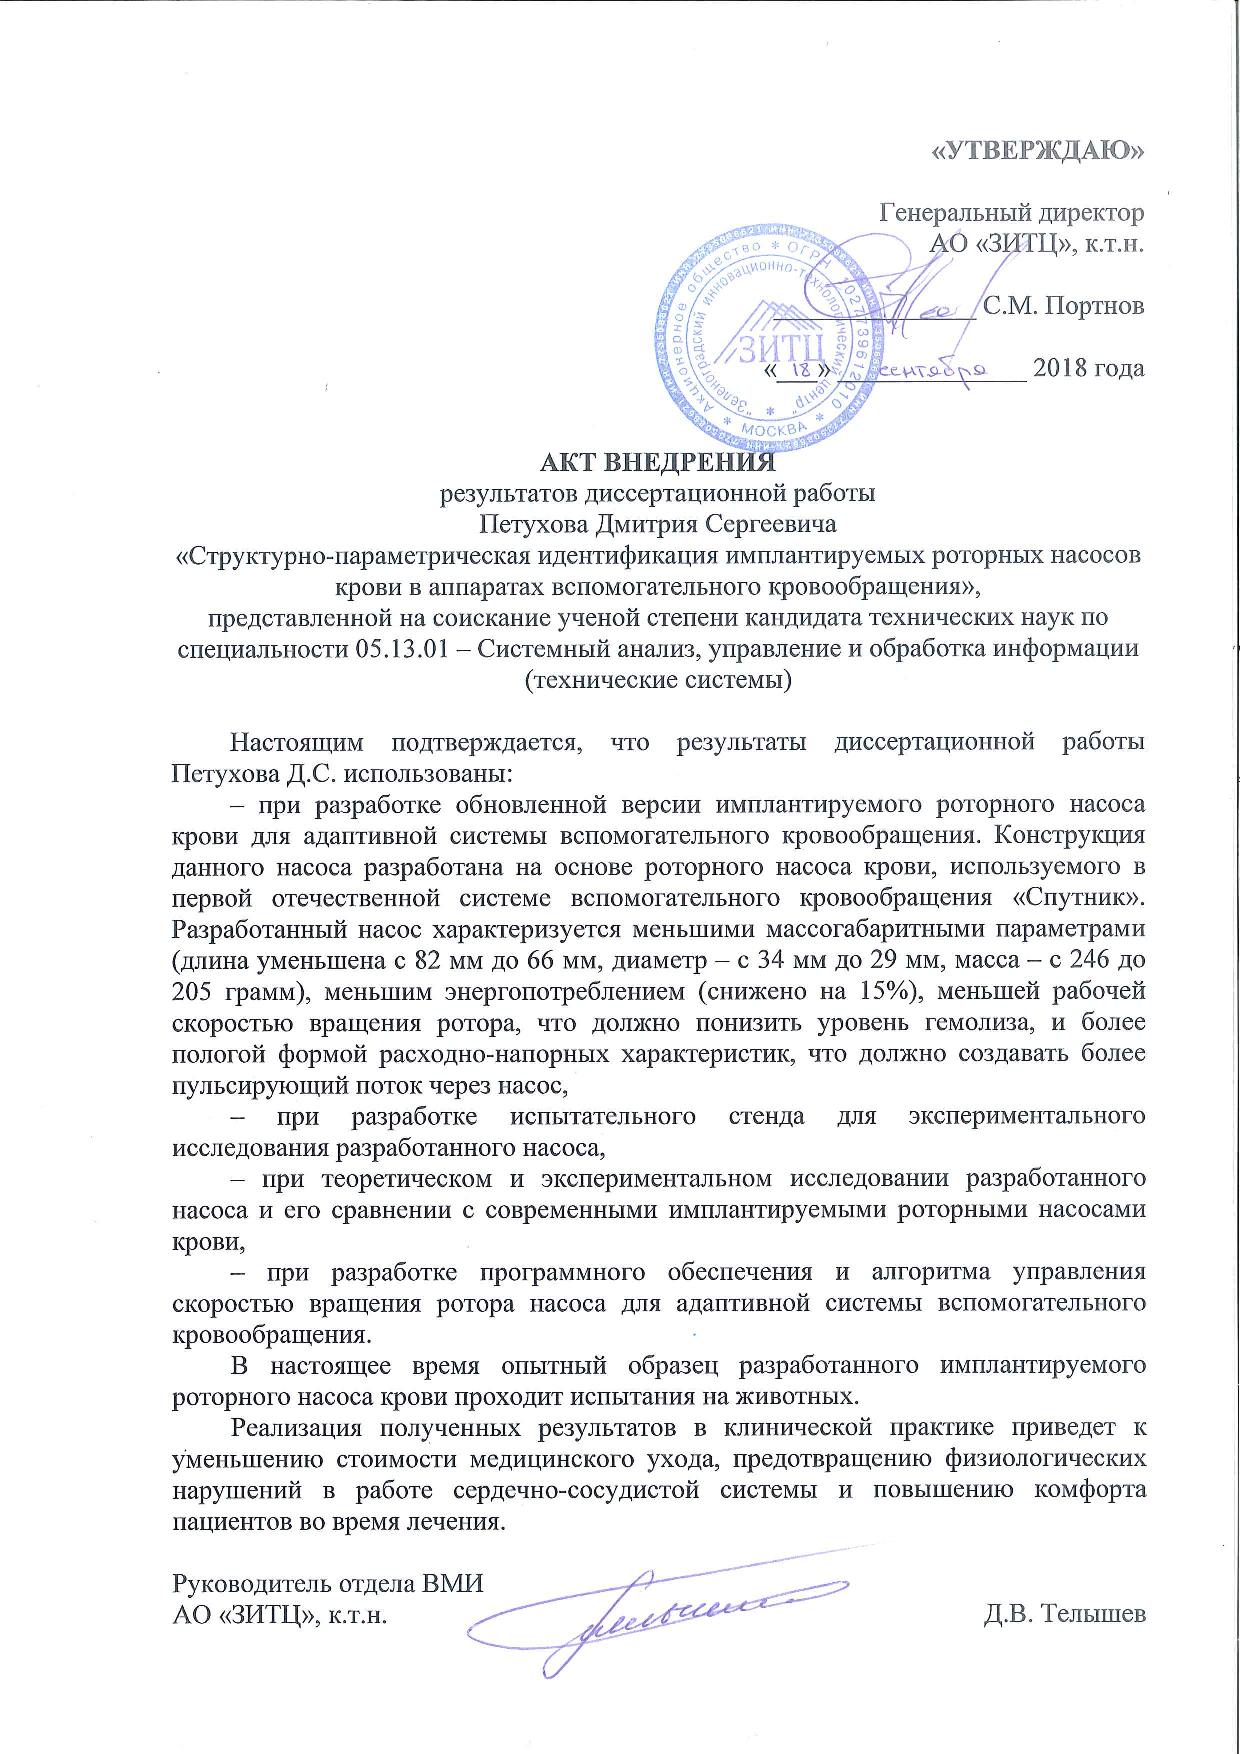
\includegraphics [scale=0.67] {../images/act_1}
  %\caption{Статические расходно-напорные характеристики роторного насоса крови} 
  %\label{img:full_static_model}  
\end{figure}
\newpage
\begin{figure}[ht] 
  \center
  \vskip\baselineskip

 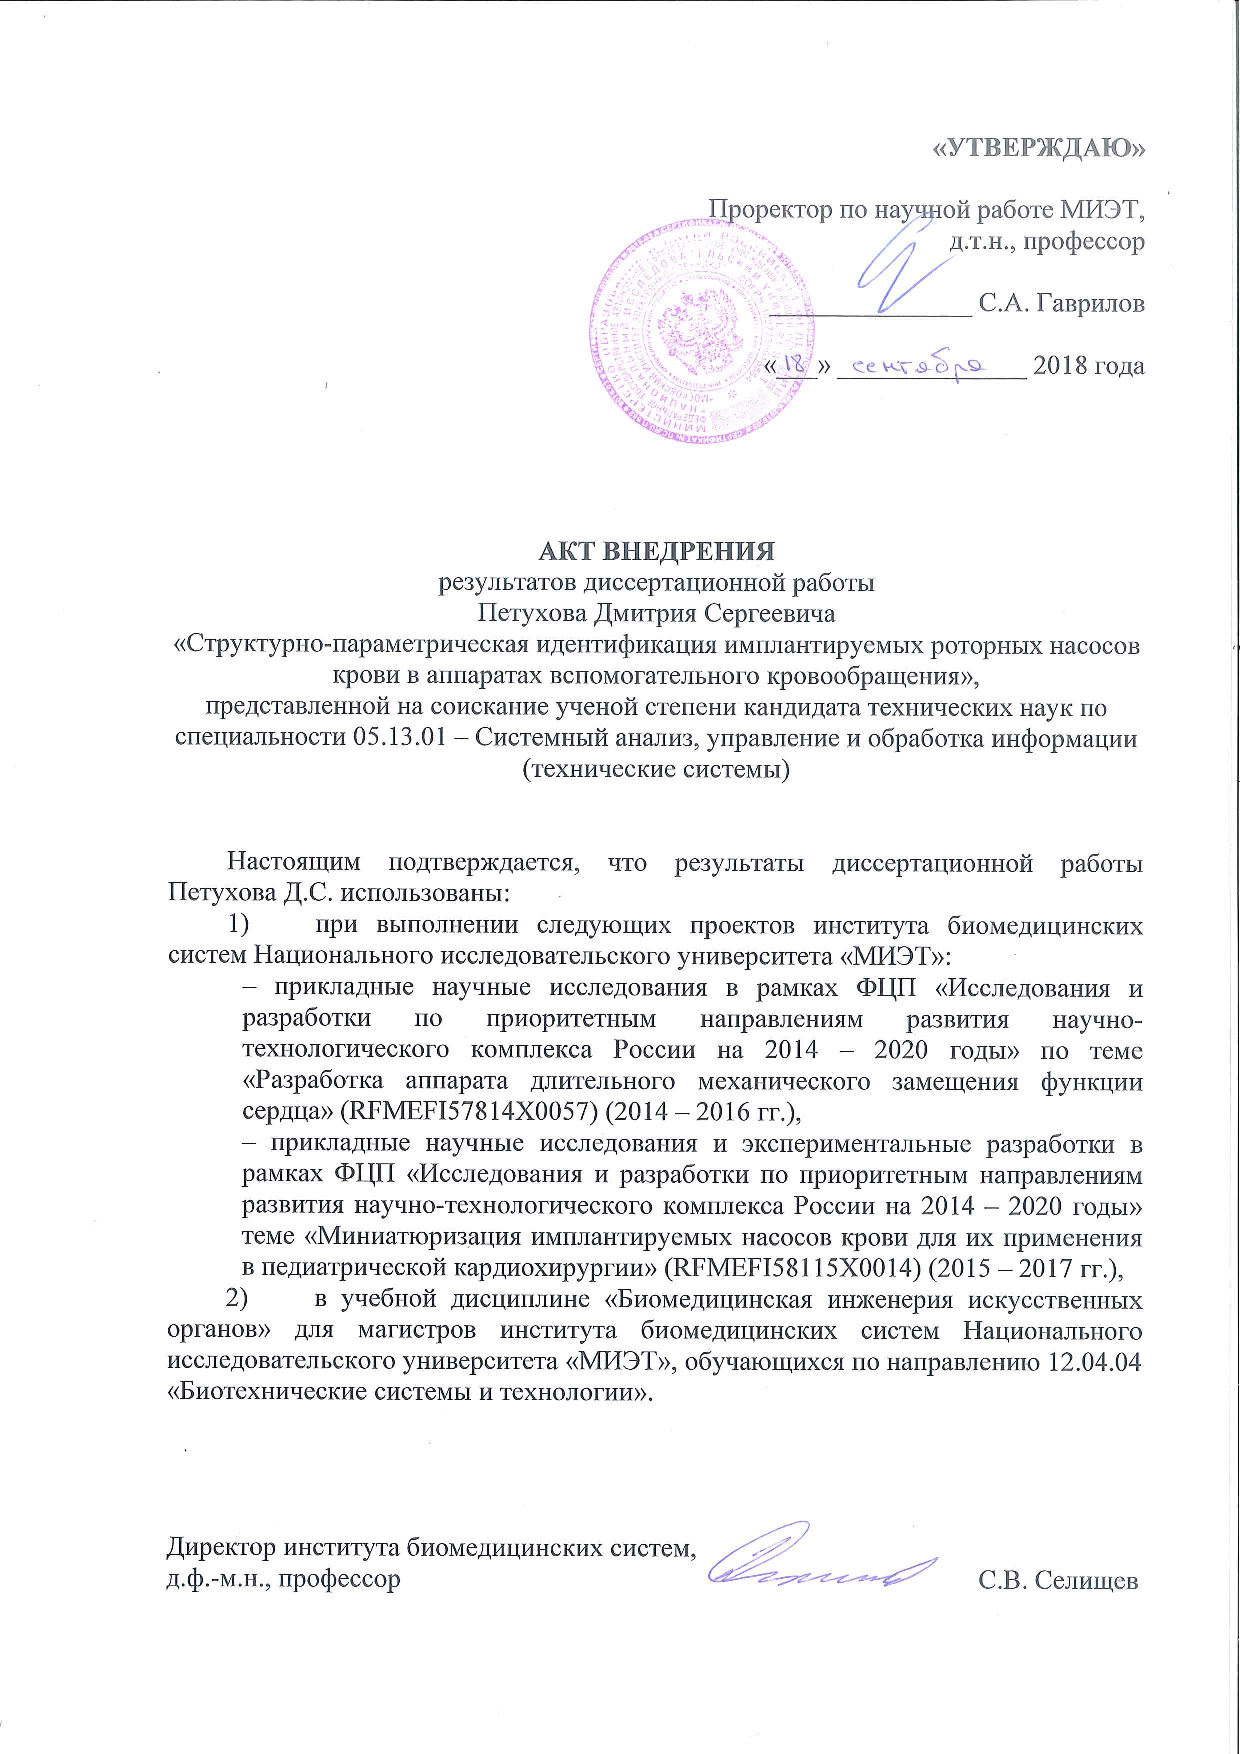
\includegraphics [scale=0.67] {../images/act_2}
 %\caption{Статические расходно-напорные характеристики роторного насоса крови} 
 %\label{img:full_static_model}  
\end{figure}
\clearpage
\newpage

% ----------------------------------------------------------------------------------------------------------------------------------------------------------------------------------------------------------------------------
% ----------------------------------------------------------------------------------------------------------------------------------------------------------------------------------------------------------------------------

\chapter{Программный код процедуры оптимизации} \label{AppendixA}

%~\ref{list:optimization_routine}.

\begin{lstlisting}[language=Python,caption={Процедура оптимизации на основе алгоритма Левенберга-Марквардта на языке программирования Python},label={list:optimization_routine}]

#!/usr/bin/env python2
from numpy import e, exp, linalg, dot, eye, diag, asarray
from numpy import zeros, ones

Vart = 500e-3; Vven = 80e-3
Cart = 4e-6; Cven = 5e-6
Rart = 2e+3; Rven = 1e+3

# -------------------------------------------------------

p1 = [Rart, Cart, Vart, Rven, Cven, Vven]
p_t = '[Rart, Cart, Vart, Rven, Cven, Vven]'

p_t = p_t[1:-1].replace(" ", "").split(',')

np = len(p1) # the number of parameters

v_i = ones(np)

# -------------------------------------------------------

dx = 1e-3
lmd = 200.0 # lambda
a = 1
bk = 1 #0.95

PCWP = 4 # Pulmonary Capillary Wedge Pressure
PA = 14.0 # Pulmonary Artery
PLV = 126 # Left Ventricular Pressure 
EF = 48 # Ejection Fraction
EDV = 77 # End Diastolic Volume

T = [PCWP,PA,EF,EDV,PLV]

nf = len(T) # the number of function values

r_old = zeros(nf); r = zeros(nf); rr = zeros(nf)

J = zeros(( nf,np ))

for k in range(0,1001):

  print('#--------------\n\
# %s | sum of residuals: %s \n#------------'\
     %(k,abs(asarray(r)).sum())) 

  print('v_i = %s' %list(v_i)) 

  print('#---------------------------------------')
  for v in range(0,np):
    print('%s\t=\t%s' %(p_t[v],v_i[v]) )
  print('#---------------------------------------')

  # -------------------------------------------------------

  p_i = v_i * p1

  M = solve_system(p_i,'plot')

  print('Target values\t|\t\t Model values \t\t|\t Residual') 

  for n in range(0,nf):
    r[n] = M[n] - T[n]

  # -------------------------------------------------------

  print('#-------------------------------------')
  for f in range(0,nf):
    print('\t\t%s\t\t|\t\t%s\t\t|\t\t%s' %(T[f],M[f],r[f]) )

  # -------------------------------------------------------

  vv_i = ones(np)

  for j in range(0,np):

    vv_i[:] = v_i[:]

    vv_i[j] = vv_i[j] + dx

    pp_i = vv_i * p1

    MM = solve_system(pp_i,' ')

    for m in range(0,nf):
      rr[m] = MM[m] - T[m] 

    for i in range(0,nf):
      J[i,j] = (rr[i] - r[i])/dx

  # -------------------------------------------------------

  JT = J.T
  b = dot(-JT,r)
  A = dot(JT,J)

  r = asarray(r)

  # -------------------------------------------------------

  I = eye(np)         

  if abs(r).sum() > abs(r_old).sum():
    lmd = lmd*a
  else:
    lmd = lmd*bk

  AJ = A + lmd*I

  s = linalg.lstsq(AJ,b)[0]

  r_old[:] = r[:]

  # -------------------------------------------------------

  for i in range(0,np):

    if v_i[i] + s[i] <= 0:
      # print i,s[i]
      s[i] = s[i]/10.

    if v_i[i] + s[i] <= 0.25:
      pass
    else:
      v_i[i] = v_i[i] + s[i]

  # -------------------------------------------------------

\end{lstlisting}

\begin{lstlisting}[language=Python,caption={Процедура оптимизации на основе алгоритма дифференциальной эволюции на языке программирования Python},label={list:optimization_routine_diff}]

#!/usr/bin/env python2
# -*- coding: utf-8 -*-

from numpy import append, zeros, sum, mean, sqrt, isnan
import matplotlib.pyplot as plt
from scipy import optimize
from scipy.io import whosmat, loadmat

data = loadmat('053.mat') # Contractility Factor = 0.5

times         = data['time'][0]         # s
PumpSpeed_ref = data['pumpSpeed_ref'][0]    
# pump rotational speed reference [1/min]
PumpFlow      = data['pumpFlow_meas'][0]    
# pump flow measurement [L/min]
Pin_ref       = data['pIn_ref'][0]       
# pump inlet presssure measurement [mmHg]
Pout_ref      = data['pOut_ref'][0]      
# pump outlet pressure measurement [mmHg]

PressureHead = Pout_ref - Pin_ref

PS = []; PF = []; PH = []; PT = []
PF = {}; PH = {}; PT = {}
ti = 2000 # time interval 2 s

for i in range(len(PumpSpeed_ref)):
  if PumpSpeed_ref[i] > PumpSpeed_ref[i-1]:
    if PumpSpeed_ref[i-1] >= 6200:
      PS.append(PumpSpeed_ref[i-1])
      PF[PumpSpeed_ref[i-1]] = (PumpFlow[i-3001-ti:i-3001])
      PH[PumpSpeed_ref[i-1]] = (PressureHead[i-3001-ti:i-3001])
      PT[PumpSpeed_ref[i-1]] = (times[i-3001-ti:i-3001])

# --------------------------------------------

M = []; dt = 0.001

# --------------------------------------------

def fpump(pp,speed,auxiliary_function):

    M = []

    a = pp[0]
    b = pp[1]
    c = pp[2]
    L = pp[3]
    d = pp[4]

    for vvad in speed:

      Q = zeros(len(PF[vvad]))
      H = zeros(len(PH[vvad]))

      Q[-1] = PF[vvad][0]

      for i in range(len(PH[vvad])):

        # --------------------------------------------

        H[i] = PH[vvad][i]

        Qe = zeros(3); Qe[0] = Q[i-1] 

        for j in range(0,2):
          Qe[j+1] = Qe[j] + dt*( \
            ( \
              a*Qe[j] + b*vvad**2 + c*H[i] + d*eval(auxiliary_function) #
            ) / L )

        Q[i] = Qe[1]

        # --------------------------------------------
      
      M += Q.tolist()

    return M

# --------------------------------------------

pump_sp = [7000,8000,9000]

# --------------------------------------------

def o_func(params, aux_func):

  T = []
  for i in pump_sp:
      for j in ( range(len( PF[i] ) ) ):
          T = append(T,PF[i][j])

  nf = len(T) # the number of function values

  r = zeros(nf)

  M = fpump(params,pump_sp,aux_func)

  for n in range(0,nf):
    r[n] = M[n] - T[n]

  return abs(r).sum()

# --------------------------------------------

af = open('auxiliary functions.txt','r')
aux_func = af.readlines()
print aux_func,len(aux_func)

strategies = ['best1bin','best1exp','rand1exp','randtobest1exp','best2exp','rand2exp','randtobest1bin',\
'best2bin','rand2bin','rand1bin']

for af in aux_func:
  print af.strip()

  start = time()

  # initial bounds for basic equation
  bounds = [(-10.0, 10.0), (-10.0, 10.0), (-10.0, 10.0), (-1e+5, 1e+5), (-0.01, 0.01)] 
  bounds = [(-10.0, 10.0), (-10.0, 10.0), (-10.0, 10.0), (-1e+4, 1e+4)] 
  nb = 1e+2 #1e+0 # initial bounds for 'd' coefficient

  # --------------------------------------------
 
  testVar = 0

  def print_fun(*args,**kwargs):
    global testVar
    
    if isnan(kwargs['convergence']) == True:
      print('Try no. %d' %testVar)
      testVar += 1

    if testVar >= 5:
      testVar = 0
      return True 

  # --------------------------------------------

  for b in range(10000):

    new_bounds = bounds[:]
    new_bounds.append( (-nb,nb) )
    print new_bounds

    for st in strategies:

      print('# --------------- %s ---------------' %st) 

      result = optimize.differential_evolution( o_func,new_bounds,args=[af.strip()],strategy=st,\
      tol=0.001,popsize=20,mutation=0.6,recombination=0.6,disp=True,callback=print_fun,polish=False )
    
      print result.message
      if result.message == 'Optimization terminated successfully.':
        break

    print('The Continued ...',nb)

    if result.message == 'Optimization terminated successfully.':
      break # do some break
    else:
      nb = nb/10. # new bounds determination

  # --------------------------------------------

  print('Ok, continue now ...')

  print result
  print result.fun
  print result.x
  print result.nit

# --------------------------------------------
# goodness of fit

  T = []
  for k in pump_sp:
      for n in ( range(len( PF[k] ) ) ):
          T = append(T,PF[k][n])

  M = fpump( result.x,pump_sp,af.strip() )

  nf = len(T); r = zeros(nf); RMSE = zeros(nf); MN = zeros(nf)

  for n in range(0,nf):
    RMSE[n] = (M[n] - T[n])**2

  rmse = sqrt(RMSE.sum()/nf)

  # --------------------------- R_squared

  Tmean = mean(T)
  for n in range(0,nf):
    MN[n] = (T[n] - Tmean)**2

  SSE = RMSE.sum()
  SST = sum(MN)

  rs = (1-(SSE/SST) )

# ----------------------------------------------

  elapsed = time() - start;

  rf = open('results_general_S1.txt','a')
  rf.write('%s \t %g \t %g \t %g \t %g \t %g \t %g \t %s\n'%(af.strip(),elapsed/60.,result.nit,result.nfev,result.fun,rs,rmse,result.x) )
  rf.close()

# --------------------------------------------

  for n in pump_sp: 
    plt.plot(range(len(PT[n])),PF[n],'k:', lw=2.0 )

  k = 0

  for n in pump_sp: # model
    plt.plot(range( len(PT[n] )),M[ k*len(PT[n]):(k+1)*len(PT[n]) ])
    k += 1

  # --------------------------------------------

  plt.ylabel(u'Перепад давления, мм рт. ст.')
  plt.xlabel(u'Расход, л/мин')
  plt.grid(True)
  plt.savefig( '%s.png' %af.strip().replace('**','^').replace('*','_') )
  plt.clf()

\end{lstlisting}

% ----------------------------------------------------------------------------------------------------------------------------------------------------------------------------------------------------------------------------
% ----------------------------------------------------------------------------------------------------------------------------------------------------------------------------------------------------------------------------

\chapter{Программный код математических моделей сердечно-сосудистой системы} \label{AppendixB}

\begin{lstlisting}[language=Python,caption={Математическая модель сердечно-сосудистой системы на языке программирования Python},label={list:cardiovascular_system_model}]
#!/usr/bin/env python2
# -*- coding: utf-8 -*-

from numpy import e, exp, zeros, pi, ones, asarray, amax, amin
from pv import pv_evaluation
import matplotlib.pyplot as plt
from matplotlib import rcParams

# -------------------------------------------------------

N = 30000

Plv = zeros(N); Prv = zeros(N) # left and right ventricular pressures
Pao = zeros(N) # aortic pressure
Pcv = zeros(N) # central venous pressure
Ppa = zeros(N) # pulmonary artery pressure
Pcw = zeros(N) # pulmonary capillary wedge pressure 
Pt  = zeros(N) # test pressure

t = zeros(N); dt = 0.001

HR = 80; t_cycle = 60.0/HR

# -------------------------------------------------------

def solve_system(param, speed, draw):

  Rart_L1 = param[0]; Rart_L2 = param[1]; Rart_L3 = param[2]
  Rart_L4 = param[3]; Rart_L5 = param[4]
  Rp_L   = param[5]
  Rven_L = param[6]   

  Rart_R1 = param[7]; Rart_R2 = param[8]; Rart_R3 = param[9]
  Rart_R4 = param[10]; Rart_R5 = param[11]
  Rp_R   = param[12]    
  Rven_R = param[13]  

  Cart_L1 = param[14]; Cart_L2 = param[15]; Cart_L3 = param[16]
  Cart_L4 = param[17]; Cart_L5 = param[18]
  Cven_L = param[19]
  Cart_R1 = param[20]; Cart_R2 = param[21]; Cart_R3 = param[22]
  Cart_R4 = param[23]; Cart_R5 = param[24]
  Cven_R = param[25]

  Lart_L1 = param[26]; Lart_L2 = param[27]; Lart_L3 = param[28]
  Lart_L4 = param[29]; Lart_L5 = param[30]
  Lven_L = param[31]

  Lart_R1 = param[32]; Lart_R2 = param[33] ; Lart_R3 = param[34]
  Lart_R4 = param[35]; Lart_R5 = param[36]
  Lven_R = param[37]

  Vart0_L = param[38] 
  Vven0_L = param[39]
  Vart0_R = param[40]
  Vven0_R = param[41]

  Vlv = zeros(N); Vlv[0] = param[42] 
  Vrv = zeros(N); Vrv[0] = param[43]

  sar = param[44]

  # -------------------------------------------------------

  Part_L1 = Vart0_L/Cart_L1; Part_L2 = Vart0_L/Cart_L2
  Part_L3 = Vart0_L/Cart_L3; Part_L4 = Vart0_L/Cart_L4; Part_L5 = Vart0_L/Cart_L5
  Pven_L = Vven0_L/Cven_L   # Pa

  Part_R1 = Vart0_R/Cart_R1; Part_R2 = Vart0_R/Cart_R2
  Part_R3 = Vart0_R/Cart_R3; Part_R4 = Vart0_R/Cart_R4; Part_R5 = Vart0_R/Cart_R5
  Pven_R = Vven0_R/Cven_R   # Pa

  Rmv = 1e-3; Rav = 1e-3; Rtr = 1e-3; Rpv = 1e-3

  Vart_L = zeros((N,5));  Vart_L[0,:] = Vart0_L
  Vven_L = zeros(N);      Vven_L[0] = Vven0_L
  Vart_R = zeros((N,5));  Vart_R[0,:] = Vart0_R
  Vven_R = zeros(N);      Vven_R[0] = Vven0_R

  q_art_L1 = zeros(N); q_art_L2 = zeros(N); q_art_L3 = zeros(N)
  q_art_L4 = zeros(N); q_art_L5 = zeros(N); 
  q_ven_L = zeros(N)
  q_art_R1 = zeros(N); q_art_R2 = zeros(N); q_art_R3 = zeros(N)
  q_art_R4 = zeros(N); q_art_R5 = zeros(N); 
  q_ven_R = zeros(N)

  q = zeros((N,4))
  ta = 0; i = 0
  q_vad = zeros(N)

  # -------------------------------------------------------

  q_art_L1[i+1] = (dt*( Plv[i] - Part_L1) + Lart_L1*q_art_L1[i]) / (Lart_L1 + dt*(Rart_L1 + Rav)) 
  q_art_L2[i+1] = (dt*(Part_L1 - Part_L2) + Lart_L2*q_art_L2[i]) / (Lart_L2 + dt*Rart_L2) 
  q_art_L3[i+1] = (dt*(Part_L2 - Part_L3) + Lart_L3*q_art_L3[i]) / (Lart_L3 + dt*Rart_L3) 
  q_art_L4[i+1] = (dt*(Part_L3 - Part_L4) + Lart_L4*q_art_L4[i]) / (Lart_L4 + dt*Rart_L4) 
  q_art_L5[i+1] = (dt*(Part_L4 - Part_L5) + Lart_L5*q_art_L5[i]) / (Lart_L5 + dt*Rart_L5) 

  q_ven_L[i+1] = (dt*(Pven_L - Prv[i]) + Lven_L*q_ven_L[i]) / (Lven_L + dt*(Rven_L + Rtr))

  q_art_R1[i+1] = (dt*( Prv[i] - Part_R1) + Lart_R1*q_art_R1[i]) / (Lart_R1 + dt*(Rart_R1 + Rpv)) 
  q_art_R2[i+1] = (dt*(Part_R1 - Part_R2) + Lart_R2*q_art_R2[i]) / (Lart_R2 + dt*Rart_R2) 
  q_art_R3[i+1] = (dt*(Part_R2 - Part_R3) + Lart_R3*q_art_R3[i]) / (Lart_R3 + dt*Rart_R3) 
  q_art_R4[i+1] = (dt*(Part_R3 - Part_R4) + Lart_R4*q_art_R4[i]) / (Lart_R4 + dt*Rart_R4) 
  q_art_R5[i+1] = (dt*(Part_R4 - Part_R5) + Lart_R5*q_art_R5[i]) / (Lart_R5 + dt*Rart_R5) 

  q_ven_R[i+1] = (dt*(Pven_R - Plv[i]) + Lven_R*q_ven_R[i]) / (Lven_R + dt*(Rven_R + Rmv))

  # -------------------------------------------------------

  q_art_L1[i+2] = ( 2*dt*( Plv[i] - Part_L1) + Lart_L1*(4*q_art_L1[i+1] - q_art_L1[i]) ) / (3*Lart_L1 + 2*dt*(Rart_L1 + Rav)) 
  q_art_L2[i+2] = ( 2*dt*(Part_L1 - Part_L2) + Lart_L1*(4*q_art_L2[i+1] - q_art_L2[i]) ) / (3*Lart_L1 + 2*dt*Rart_L1)
  q_art_L3[i+2] = ( 2*dt*(Part_L2 - Part_L3) + Lart_L1*(4*q_art_L3[i+1] - q_art_L3[i]) ) / (3*Lart_L1 + 2*dt*Rart_L1)
  q_art_L4[i+2] = ( 2*dt*(Part_L3 - Part_L4) + Lart_L1*(4*q_art_L4[i+1] - q_art_L4[i]) ) / (3*Lart_L1 + 2*dt*Rart_L1)
  q_art_L5[i+2] = ( 2*dt*(Part_L4 - Part_L5) + Lart_L1*(4*q_art_L5[i+1] - q_art_L5[i]) ) / (3*Lart_L1 + 2*dt*Rart_L1)

  q_ven_L[i+2] = ( 2*dt*(Pven_L - Prv[i] ) + Lven_L*(4*q_ven_L[i+1] - q_ven_L[i]) ) / (3*Lven_L + 2*dt*(Rven_L + Rtr)) 

  q_art_R1[i+2] = ( 2*dt*( Prv[i] - Part_R1) + Lart_R1*(4*q_art_R1[i+1] - q_art_R1[i]) ) / (3*Lart_R1 + 2*dt*(Rart_R1 + Rpv)) 
  q_art_R2[i+2] = ( 2*dt*(Part_R1 - Part_R2) + Lart_R1*(4*q_art_R2[i+1] - q_art_R2[i]) ) / (3*Lart_R1 + 2*dt*Rart_R1)
  q_art_R3[i+2] = ( 2*dt*(Part_R2 - Part_R3) + Lart_R1*(4*q_art_R3[i+1] - q_art_R3[i]) ) / (3*Lart_R1 + 2*dt*Rart_R1)
  q_art_R4[i+2] = ( 2*dt*(Part_R3 - Part_R4) + Lart_R1*(4*q_art_R4[i+1] - q_art_R4[i]) ) / (3*Lart_R1 + 2*dt*Rart_R1)
  q_art_R5[i+2] = ( 2*dt*(Part_R4 - Part_R5) + Lart_R1*(4*q_art_R5[i+1] - q_art_R5[i]) ) / (3*Lart_R1 + 2*dt*Rart_R1)

  q_ven_R[i+2] = ( 2*dt*(Pven_R - Plv[i] ) + Lven_R*(4*q_ven_R[i+1] - q_ven_R[i]) ) / (3*Lven_R + 2*dt*(Rven_R + Rmv)) 

  # -------------------------------------------------------

  q_art_L1[i+3] = ( 6*dt*( Plv[i] - Part_L1) + Lart_L1*(18*q_art_L1[i+2] - 9*q_art_L1[i+1] + 2*q_art_L1[i]) ) / (11*Lart_L1 + 6*dt*(Rart_L1 + Rav)) 
  q_art_L2[i+3] = ( 6*dt*(Part_L1 - Part_L2) + Lart_L2*(18*q_art_L2[i+2] - 9*q_art_L2[i+1] + 2*q_art_L2[i]) ) / (11*Lart_L2 + 6*dt*Rart_L2)
  q_art_L3[i+3] = ( 6*dt*(Part_L2 - Part_L3) + Lart_L3*(18*q_art_L3[i+2] - 9*q_art_L3[i+1] + 2*q_art_L3[i]) ) / (11*Lart_L3 + 6*dt*Rart_L3)
  q_art_L4[i+3] = ( 6*dt*(Part_L3 - Part_L4) + Lart_L4*(18*q_art_L4[i+2] - 9*q_art_L4[i+1] + 2*q_art_L4[i]) ) / (11*Lart_L4 + 6*dt*Rart_L4)
  q_art_L5[i+3] = ( 6*dt*(Part_L4 - Part_L5) + Lart_L5*(18*q_art_L5[i+2] - 9*q_art_L5[i+1] + 2*q_art_L5[i]) ) / (11*Lart_L5 + 6*dt*Rart_L5)

  q_ven_L[i+3] = ( 6*dt*(Pven_L - Prv[i] ) + Lven_L*(18*q_ven_L[i+2] - 9*q_ven_L[i+1] + 2*q_ven_L[i]) ) / (11*Lven_L + 6*dt*(Rven_L + Rtr))

  q_art_R1[i+3] = ( 6*dt*( Prv[i] - Part_R1) + Lart_R1*(18*q_art_R1[i+2] - 9*q_art_R1[i+1] + 2*q_art_R1[i]) ) / (11*Lart_R1 + 6*dt*(Rart_R1 + Rpv)) 
  q_art_R2[i+3] = ( 6*dt*(Part_R1 - Part_R2) + Lart_R2*(18*q_art_R2[i+2] - 9*q_art_R2[i+1] + 2*q_art_R2[i]) ) / (11*Lart_R2 + 6*dt*Rart_R2)
  q_art_R3[i+3] = ( 6*dt*(Part_R2 - Part_R3) + Lart_R3*(18*q_art_R3[i+2] - 9*q_art_R3[i+1] + 2*q_art_R3[i]) ) / (11*Lart_R3 + 6*dt*Rart_R3)
  q_art_R4[i+3] = ( 6*dt*(Part_R3 - Part_R4) + Lart_R4*(18*q_art_R4[i+2] - 9*q_art_R4[i+1] + 2*q_art_R4[i]) ) / (11*Lart_R4 + 6*dt*Rart_R4)
  q_art_R5[i+3] = ( 6*dt*(Part_R4 - Part_R5) + Lart_R5*(18*q_art_R5[i+2] - 9*q_art_R5[i+1] + 2*q_art_R5[i]) ) / (11*Lart_R5 + 6*dt*Rart_R5)
  
  q_ven_R[i+3] = ( 6*dt*(Pven_R - Plv[i] ) + Lven_R*(18*q_ven_R[i+2] - 9*q_ven_R[i+1] + 2*q_ven_R[i]) ) / (11*Lven_R + 6*dt*(Rven_R + Rmv)) 

  # -------------------------------------------------------

  q_art_L1[i+4] = ( 12*dt*( Plv[i] - Part_L1) + Lart_L1*(48*q_art_L1[i+3] - 36*q_art_L1[i+2] + 16*q_art_L1[i+1] - 3*q_art_L1[i]) ) / (25*Lart_L1 + 12*dt*(Rart_L1 + Rav)) 
  q_art_L2[i+4] = ( 12*dt*(Part_L1 - Part_L2) + Lart_L2*(48*q_art_L2[i+3] - 36*q_art_L2[i+2] + 16*q_art_L2[i+1] - 3*q_art_L2[i]) ) / (25*Lart_L2 + 12*dt*Rart_L2)
  q_art_L3[i+4] = ( 12*dt*(Part_L2 - Part_L3) + Lart_L3*(48*q_art_L3[i+3] - 36*q_art_L3[i+2] + 16*q_art_L3[i+1] - 3*q_art_L3[i]) ) / (25*Lart_L3 + 12*dt*Rart_L3)
  q_art_L4[i+4] = ( 12*dt*(Part_L3 - Part_L4) + Lart_L4*(48*q_art_L4[i+3] - 36*q_art_L4[i+2] + 16*q_art_L4[i+1] - 3*q_art_L4[i]) ) / (25*Lart_L4 + 12*dt*Rart_L4)
  q_art_L5[i+4] = ( 12*dt*(Part_L4 - Part_L5) + Lart_L5*(48*q_art_L5[i+3] - 36*q_art_L5[i+2] + 16*q_art_L5[i+1] - 3*q_art_L5[i]) ) / (25*Lart_L5 + 12*dt*Rart_L5)
     
  q_ven_L[i+4] = ( 12*dt*(Pven_L - Prv[i] ) + Lven_L*(48*q_ven_L[i+3] - 36*q_ven_L[i+2] + 16*q_ven_L[i+1] - 3*q_ven_L[i]) ) / (25*Lven_L + 12*dt*(Rven_L + Rtr)) 

  q_art_R1[i+4] = ( 12*dt*( Prv[i] - Part_R1) + Lart_R1*(48*q_art_R1[i+3] - 36*q_art_R1[i+2] + 16*q_art_R1[i+1] - 3*q_art_R1[i]) ) / (25*Lart_R1 + 12*dt*(Rart_R1 + Rpv)) 
  q_art_R2[i+4] = ( 12*dt*(Part_R1 - Part_R2) + Lart_R2*(48*q_art_R2[i+3] - 36*q_art_R2[i+2] + 16*q_art_R2[i+1] - 3*q_art_R2[i]) ) / (25*Lart_R2 + 12*dt*Rart_R2)
  q_art_R3[i+4] = ( 12*dt*(Part_R2 - Part_R3) + Lart_R3*(48*q_art_R3[i+3] - 36*q_art_R3[i+2] + 16*q_art_R3[i+1] - 3*q_art_R3[i]) ) / (25*Lart_R3 + 12*dt*Rart_R3)
  q_art_R4[i+4] = ( 12*dt*(Part_R3 - Part_R4) + Lart_R4*(48*q_art_R4[i+3] - 36*q_art_R4[i+2] + 16*q_art_R4[i+1] - 3*q_art_R4[i]) ) / (25*Lart_R4 + 12*dt*Rart_R4)
  q_art_R5[i+4] = ( 12*dt*(Part_R4 - Part_R5) + Lart_R5*(48*q_art_R5[i+3] - 36*q_art_R5[i+2] + 16*q_art_R5[i+1] - 3*q_art_R5[i]) ) / (25*Lart_R5 + 12*dt*Rart_R5)

  q_ven_R[i+4] = ( 12*dt*(Pven_R - Plv[i] ) + Lven_R*(48*q_ven_R[i+3] - 36*q_ven_R[i+2] + 16*q_ven_R[i+1] - 3*q_ven_R[i]) ) / (25*Lven_R + 12*dt*(Rven_R + Rmv)) 

  # -------------------------------------------------------
  
  q_art_L1[i+5] = ( 60*dt*( Plv[i] - Part_L1) + Lart_L1*(300*q_art_L1[i] - 300*q_art_L1[i-1] + 200*q_art_L1[i-2] - 75*q_art_L1[i-3] + 12*q_art_L1[i-4]) ) / (137*Lart_L1 + 60*dt*(Rart_L1 + Rav)) 
  q_art_L2[i+5] = ( 60*dt*(Part_L1 - Part_L2) + Lart_L2*(300*q_art_L2[i] - 300*q_art_L2[i-1] + 200*q_art_L2[i-2] - 75*q_art_L2[i-3] + 12*q_art_L2[i-4]) ) / (137*Lart_L2 + 60*dt*Rart_L2)
  q_art_L3[i+5] = ( 60*dt*(Part_L2 - Part_L3) + Lart_L3*(300*q_art_L3[i] - 300*q_art_L3[i-1] + 200*q_art_L3[i-2] - 75*q_art_L3[i-3] + 12*q_art_L3[i-4]) ) / (137*Lart_L3 + 60*dt*Rart_L3)
  q_art_L4[i+5] = ( 60*dt*(Part_L3 - Part_L4) + Lart_L4*(300*q_art_L4[i] - 300*q_art_L4[i-1] + 200*q_art_L4[i-2] - 75*q_art_L4[i-3] + 12*q_art_L4[i-4]) ) / (137*Lart_L4 + 60*dt*Rart_L4)
  q_art_L5[i+5] = ( 60*dt*(Part_L4 - Part_L5) + Lart_L5*(300*q_art_L5[i] - 300*q_art_L5[i-1] + 200*q_art_L5[i-2] - 75*q_art_L5[i-3] + 12*q_art_L5[i-4]) ) / (137*Lart_L5 + 60*dt*Rart_L5)
      
  q_ven_L[i+5] = ( 60*dt*(Pven_L - Prv[i] ) + Lven_L*(300*q_ven_L[i] - 300*q_ven_L[i-1] + 200*q_ven_L[i-2] - 75*q_ven_L[i-3] + 12*q_ven_L[i-4]) ) / (137*Lven_L + 60*dt*(Rven_L + Rtr)) 

  q_art_R1[i+5] = ( 60*dt*( Prv[i] - Part_R1) + Lart_R1*(300*q_art_R1[i] - 300*q_art_R1[i-1] + 200*q_art_R1[i-2] - 75*q_art_R1[i-3] + 12*q_art_R1[i-4]) ) / (137*Lart_R1 + 60*dt*(Rart_R1 + Rpv)) 
  q_art_R2[i+5] = ( 60*dt*(Part_R1 - Part_R2) + Lart_R2*(300*q_art_R2[i] - 300*q_art_R2[i-1] + 200*q_art_R2[i-2] - 75*q_art_R2[i-3] + 12*q_art_R2[i-4]) ) / (137*Lart_R2 + 60*dt*Rart_R2)
  q_art_R3[i+5] = ( 60*dt*(Part_R2 - Part_R3) + Lart_R3*(300*q_art_R3[i] - 300*q_art_R3[i-1] + 200*q_art_R3[i-2] - 75*q_art_R3[i-3] + 12*q_art_R3[i-4]) ) / (137*Lart_R3 + 60*dt*Rart_R3)
  q_art_R4[i+5] = ( 60*dt*(Part_R3 - Part_R4) + Lart_R4*(300*q_art_R4[i] - 300*q_art_R4[i-1] + 200*q_art_R4[i-2] - 75*q_art_R4[i-3] + 12*q_art_R4[i-4]) ) / (137*Lart_R4 + 60*dt*Rart_R4)
  q_art_R5[i+5] = ( 60*dt*(Part_R4 - Part_R5) + Lart_R5*(300*q_art_R5[i] - 300*q_art_R5[i-1] + 200*q_art_R5[i-2] - 75*q_art_R5[i-3] + 12*q_art_R5[i-4]) ) / (137*Lart_R5 + 60*dt*Rart_R5)

  q_ven_R[i+5] = ( 60*dt*(Pven_R - Plv[i] ) + Lven_R*(300*q_ven_R[i] - 300*q_ven_R[i-1] + 200*q_ven_R[i-2] - 75*q_ven_R[i-3] + 12*q_ven_R[i-4]) ) / (137*Lven_R + 60*dt*(Rven_R + Rmv)) 
  
  # -------------------------------------------------------

  for i in range(0,N-1):

    t[i+1] = (t[i] + dt)

    if (t[i+1]/(t_cycle/2.))%2 < 1:
      ta = 0
    else:
      ta = ta + dt

    q_P_L = (Part_L5 - Pven_L)/Rp_L
    q_P_R = (Part_R5 - Pven_R)/Rp_R

	 # -------------------------------------------------------

    if Plv[i] < Part_L1:
      Rav = 1e+12
    else:
      Rav = 1e-3

    # -------------------------------------------------------

    if i >= 5:

      q_art_L1[i+1] = ( 60*dt*( Plv[i] - Part_L1) + Lart_L1*(360*q_art_L1[i] - 450*q_art_L1[i-1] + 400*q_art_L1[i-2] - 225*q_art_L1[i-3] + 72*q_art_L1[i-4] - 10*q_art_L1[i-5]) ) / (147*Lart_L1 + 60*dt*(Rart_L1 + Rav)) 
      q_art_L2[i+1] = ( 60*dt*(Part_L1 - Part_L2) + Lart_L2*(360*q_art_L2[i] - 450*q_art_L2[i-1] + 400*q_art_L2[i-2] - 225*q_art_L2[i-3] + 72*q_art_L2[i-4] - 10*q_art_L2[i-5]) ) / (147*Lart_L2 + 60*dt*Rart_L2)
      q_art_L3[i+1] = ( 60*dt*(Part_L2 - Part_L3) + Lart_L3*(360*q_art_L3[i] - 450*q_art_L3[i-1] + 400*q_art_L3[i-2] - 225*q_art_L3[i-3] + 72*q_art_L3[i-4] - 10*q_art_L3[i-5]) ) / (147*Lart_L3 + 60*dt*Rart_L3)
      q_art_L4[i+1] = ( 60*dt*(Part_L3 - Part_L4) + Lart_L4*(360*q_art_L4[i] - 450*q_art_L4[i-1] + 400*q_art_L4[i-2] - 225*q_art_L4[i-3] + 72*q_art_L4[i-4] - 10*q_art_L4[i-5]) ) / (147*Lart_L4 + 60*dt*Rart_L4)
      q_art_L5[i+1] = ( 60*dt*(Part_L4 - Part_L5) + Lart_L5*(360*q_art_L5[i] - 450*q_art_L5[i-1] + 400*q_art_L5[i-2] - 225*q_art_L5[i-3] + 72*q_art_L5[i-4] - 10*q_art_L5[i-5]) ) / (147*Lart_L5 + 60*dt*Rart_L5)
         
    q[i,0] = q_art_L1[i+1]

    # -------------------------------------------------------

    if Pven_L < Prv[i]:
      Rtr = 1e+12
    else:
      Rtr = 1e-3

	 # -------------------------------------------------------

    if i >= 5:
      q_ven_L[i+1] = ( 60*dt*(Pven_L - Prv[i] ) + Lven_L*(360*q_ven_L[i] - 450*q_ven_L[i-1] + 400*q_ven_L[i-2] - 225*q_ven_L[i-3] + 72*q_ven_L[i-4] - 10*q_ven_L[i-5]) ) / (147*Lven_L + 60*dt*(Rven_L + Rtr)) 

    q[i,1] = q_ven_L[i+1]  
    
    # -------------------------------------------------------

    if Prv[i] < Part_R1:
      Rpv = 1e+12
    else:
      Rpv = 1e-3

    # -------------------------------------------------------

    if i >= 5:

      q_art_R1[i+1] = ( 60*dt*( Prv[i] - Part_R1) + Lart_R1*(360*q_art_R1[i] - 450*q_art_R1[i-1] + 400*q_art_R1[i-2] - 225*q_art_R1[i-3] + 72*q_art_R1[i-4] - 10*q_art_R1[i-5]) ) / (147*Lart_R1 + 60*dt*(Rart_R1 + Rpv)) 
      q_art_R2[i+1] = ( 60*dt*(Part_R1 - Part_R2) + Lart_R2*(360*q_art_R2[i] - 450*q_art_R2[i-1] + 400*q_art_R2[i-2] - 225*q_art_R2[i-3] + 72*q_art_R2[i-4] - 10*q_art_R2[i-5]) ) / (147*Lart_R2 + 60*dt*Rart_R2)
      q_art_R3[i+1] = ( 60*dt*(Part_R2 - Part_R3) + Lart_R3*(360*q_art_R3[i] - 450*q_art_R3[i-1] + 400*q_art_R3[i-2] - 225*q_art_R3[i-3] + 72*q_art_R3[i-4] - 10*q_art_R3[i-5]) ) / (147*Lart_R3 + 60*dt*Rart_R3)
      q_art_R4[i+1] = ( 60*dt*(Part_R3 - Part_R4) + Lart_R4*(360*q_art_R4[i] - 450*q_art_R4[i-1] + 400*q_art_R4[i-2] - 225*q_art_R4[i-3] + 72*q_art_R4[i-4] - 10*q_art_R4[i-5]) ) / (147*Lart_R4 + 60*dt*Rart_R4)
      q_art_R5[i+1] = ( 60*dt*(Part_R4 - Part_R5) + Lart_R5*(360*q_art_R5[i] - 450*q_art_R5[i-1] + 400*q_art_R5[i-2] - 225*q_art_R5[i-3] + 72*q_art_R5[i-4] - 10*q_art_R5[i-5]) ) / (147*Lart_R5 + 60*dt*Rart_R5)

    q[i,2] = q_art_R1[i+1]

    # -------------------------------------------------------

    if Pven_R < Plv[i]:
      Rmv = 1e+12
    else:
      Rmv = 1e-3

    # -------------------------------------------------------

    if i >= 5:
      q_ven_R[i+1] = ( 60*dt*(Pven_R - Plv[i] ) + Lven_R*(360*q_ven_R[i] - 450*q_ven_R[i-1] + 400*q_ven_R[i-2] - 225*q_ven_R[i-3] + 72*q_ven_R[i-4] - 10*q_ven_R[i-5]) ) / (147*Lven_R + 60*dt*(Rven_R + Rmv)) 

    q[i,3] = q_ven_R[i+1]

    # -------------------------------------------------------
    # Pump description

    dP = (-Plv[i] + Part_L1)/133.322; vvad = speed
    
    a1=-6.2332648;  a2=-0.02544392
    b1=0.53390228;  b2=-0.02391106
    c1=-0.15940332; c2=-0.01478471
    d1=1.07782859;  d2=0.04959709
    e1=-0.07888535; e2=-0.01339429
    f1=0.15683543;  f2=0.02631725
    g1=-0.65830264; g2=-0.66717543

    L = 0.2; vv = 3.6
    
    a = (a1+a2*vv); b = (b1+b2*vv); c = (c1+c2*vv)
    d = (d1+d2*vv); e = (e1+e2*vv); f = (f1+f2*vv)

    Qe = zeros(11); Qe[0] = q_vad[i-1]*60

    for j in range(0,2):

      Qe[j+1] = Qe[j] + dt*(
        (
        a*Qe[j] + b*Qe[j]**2 + c*Qe[j]**3 + d*vvad**2 + e*Qe[j]*(vvad**2) + f*vvad*(Qe[j]**2) + g1 + g2*vv - dP\
        )/L 
      )

    q_vad[i] = Qe[1]/60.

    # -------------------------------------------------------

    Vart_L[i+1,0] = Vart_L[i,0] + dt*(q_vad[i] + q_art_L1[i+1] - q_art_L2[i+1])
    Vart_L[i+1,1] = Vart_L[i,1] + dt*(q_art_L2[i+1] - q_art_L3[i+1])
    Vart_L[i+1,2] = Vart_L[i,2] + dt*(q_art_L3[i+1] - q_art_L4[i+1])
    Vart_L[i+1,3] = Vart_L[i,3] + dt*(q_art_L4[i+1] - q_art_L5[i+1])
    Vart_L[i+1,4] = Vart_L[i,4] + dt*(q_art_L5[i+1] - q_P_L)

    Part_L1 = 0 + (Vart_L[i+1,0]-Vart0_L)/Cart_L1 
    Part_L2 = 0 + (Vart_L[i+1,1]-Vart0_L)/Cart_L2 
    Part_L3 = 0 + (Vart_L[i+1,2]-Vart0_L)/Cart_L3 
    Part_L4 = 0 + (Vart_L[i+1,3]-Vart0_L)/Cart_L4 
    Part_L5 = 0 + (Vart_L[i+1,4]-Vart0_L)/Cart_L5

    Vven_L[i+1] = Vven_L[i] + dt*(q_P_L - q_ven_L[i+1]) 
    Pven_L = 0 + (Vven_L[i+1] - Vven0_L)/Cven_L

    Vart_R[i+1,0] = Vart_R[i,0] + dt*(q_art_R1[i+1] - q_art_R2[i+1])
    Vart_R[i+1,1] = Vart_R[i,1] + dt*(q_art_R2[i+1] - q_art_R3[i+1])
    Vart_R[i+1,2] = Vart_R[i,2] + dt*(q_art_R3[i+1] - q_art_R4[i+1])
    Vart_R[i+1,3] = Vart_R[i,3] + dt*(q_art_R4[i+1] - q_art_R5[i+1])
    Vart_R[i+1,4] = Vart_R[i,4] + dt*(q_art_R5[i+1] - q_P_R)

    Part_R1 = 0 + (Vart_R[i+1,0]-Vart0_R)/Cart_R1 
    Part_R2 = 0 + (Vart_R[i+1,1]-Vart0_R)/Cart_R2 
    Part_R3 = 0 + (Vart_R[i+1,2]-Vart0_R)/Cart_R3 
    Part_R4 = 0 + (Vart_R[i+1,3]-Vart0_R)/Cart_R4
    Part_R5 = 0 + (Vart_R[i+1,4]-Vart0_R)/Cart_R5 

    Vven_R[i+1] = Vven_R[i] + dt*(q_P_R - q_ven_R[i+1]) 
    Pven_R = 0 + (Vven_R[i+1] - Vven0_R)/Cven_R 

    Pao[i] = Part_L1
    Ppa[i] = Part_R1
    Pcv[i] = Prv[i] + q_ven_L[i+1]*Rtr
    Pcw[i] = Plv[i] + q_ven_R[i+1]*Rmv
    #Pt[i] = Pven_R
    
    Vlv[i+1] = Vlv[i] + dt*(q_ven_R[i+1] - q_art_L1[i+1] - q_vad[i])
    Vrv[i+1] = Vrv[i] + dt*(q_ven_L[i+1] - q_art_R1[i+1])
    Plv[i+1] = pv_evaluation(Vlv[i+1], 'lv', ta, sar, 0.5, t_cycle, Vw_lv, V0_lv)
    Prv[i+1] = pv_evaluation(Vrv[i+1], 'rv', ta, sar, 1.0, t_cycle, Vw_rv, V0_rv)

  if draw == 'plot':

    plt.subplot(313)
    plt.axis([26.5,30.0,-5,100])
    plt.plot(t,Plv/133.3,'k-',linewidth=1.5)
    plt.plot(t,Prv/133.3,'b-',linewidth=2.0)
    plt.plot(t,Pao/133.3,'r-',linewidth=0.75)
    plt.plot(t,Ppa/133.3,'c-.',linewidth=2.5)
    #plt.plot(t,Pcv/133.3,'r--',linewidth=1.0)
    #plt.plot(t,Pcw/133.3,'b--',linewidth=1.0)
    plt.legend(('Plv', 'Prv', 'Pao', 'Ppa'),'upper right', shadow=False, fancybox=False)
    plt.grid(True)

    plt.subplot(312, sharex=plt.subplot(313))
    plt.axis([26.5,30.0,0.02,0.1])
    plt.plot(t,Vlv,'r-',linewidth=2.0)
    plt.plot(t,Vrv,'b--',linewidth=2.0)
    plt.legend(('Vlv','Vrv'),'lower right', shadow=False, fancybox=False)
    plt.grid(True)
    
    plt.subplot(311, sharex=plt.subplot(313))
    plt.axis([26.5,30.0,-0.1,0.8])
    plt.plot(t,q[:,0])
    plt.plot(t,q[:,3])
    plt.legend(('q_art_L', 'q_ven_R'),'lower right', shadow=False, fancybox=False)
    plt.grid(True)
    plt.show()

  plv = amax(Plv[29770:29960])/133.322 # PLV
  sap = amax(Pao[29810:29950])/133.322 # SAP
  dap = amin(Pao[29710:29850])/133.322 # DAP
  edv = amax(Vlv[29650:29850])*1e+3 # EDV
  esv = amin(Vlv[29340:29510])*1e+3 # ESV

  sv = edv - esv

  return sv

# -------------------------------------------------------
# -------------------------------------------------------

Vart0_L = 500e-3 # L
Vven0_L = 3000e-3
Vart0_R = 80e-3
Vven0_R = 80e-3 

Cart_L1 = 4e-6; Cart_L2 = Cart_L1; Cart_L3 = Cart_L1; Cart_L4 = Cart_L1; Cart_L5 = Cart_L1 # L/Pa
Cven_L = 750e-6 
Cart_R1 = 4e-6; Cart_R2 = Cart_R1; Cart_R3 = Cart_R1; Cart_R4 = Cart_R1; Cart_R5 = Cart_R1
Cven_R = 200e-6

Rart_L1 = 15e+3; Rart_L2 = Rart_L1; Rart_L3 = Rart_L1; Rart_L4 = Rart_L1; Rart_L5 = Rart_L1 # Pa s/L
Rp_L = 126e+3   
Rven_L = 7e+3 
Rart_R1 = 3e+3; Rart_R2 = Rart_R1; Rart_R3 = Rart_R1; Rart_R4 = Rart_R1; Rart_R5 = Rart_R1
Rp_R = 20e+3    
Rven_R = 2e+3

Lart_L1 = 3.0; Lart_L2 = Lart_L1; Lart_L3 = Lart_L1; Lart_L4 = Lart_L1; Lart_L5 = Lart_L1 # Pa s^2/L
Lven_L = 3.0
Lart_R1 = 3.0; Lart_R2 = Lart_R1; Lart_R3 = Lart_R1; Lart_R4 = Lart_R1; Lart_R5 = Lart_R1
Lven_R = 3.0

Vw_lv = 300e-3    # L
Vw_rv = 100e-3    # L
V0_lv = 0.4*Vw_lv
V0_rv = 0.75*Vw_rv

Vart_L = Vart0_L
Vven_L = Vven0_L
Vart_R = Vart0_R
Vven_R = Vven0_R

sar = 55e+3

# -------------------------------------------------------

p1 = [Rart_L1,Rart_L2,Rart_L3,Rart_L4,Rart_L5,Rp_L,Rven_L,\
Rart_R1,Rart_R2,Rart_R3,Rart_R4,Rart_R5,Rp_R,Rven_R,\
Cart_L1,Cart_L2,Cart_L3,Cart_L4,Cart_L5,Cven_L,\
Cart_R1,Cart_R2,Cart_R3,Cart_R4,Cart_R5,Cven_R,\
Lart_L1,Lart_L2,Lart_L3,Lart_L4,Lart_L5,Lven_L,\
Lart_R1,Lart_R2,Lart_R3,Lart_R4,Lart_R5,Lven_R,\
Vart_L,Vven_L,Vart_R,Vven_R, V0_lv, V0_rv, sar]

p_t = '[Rart_L1,Rart_L2,Rart_L3,Rart_L4,Rart_L5,Rp_L,Rven_L,\
Rart_R1,Rart_R2,Rart_R3,Rart_R4,Rart_R5,Rp_R,Rven_R,\
Cart_L1,Cart_L2,Cart_L3,Cart_L4,Cart_L5,Cven_L,\
Cart_R1,Cart_R2,Cart_R3,Cart_R4,Cart_R5,Cven_R,\
Lart_L1,Lart_L2,Lart_L3,Lart_L4,Lart_L5,Lven_L,\
Lart_R1,Lart_R2,Lart_R3,Lart_R4,Lart_R5,Lven_R,\
Vart_L,Vven_L,Vart_R,Vven_R, V0_lv, V0_rv, sar]'

# remove brackets, remove whitespaces and create list of strings
p_t = p_t[1:-1].replace(" ", "").split(',')

np = len(p1) # the number of parameters

v_i = ones(np)

v_i = [0.057446736244404648, 0.12080933945118018, 0.51557708891696208, 1.0357810417699811, 1.060271287869758, 0.84033406019046764, 0.30211326841133845, 0.21310613995095165, 0.28955931531899554, 0.46145435968383813, 0.77440484756234174, 0.9465264404862892, 0.95668625287711806, 0.54134565361527442, 0.85805787525000099, 1.0185616722139288, 1.0003993443727075, 0.93119579177555656, 0.81353258908257642, 1.7442397377132861, 1.2984777917739705, 1.2124190153201915, 1.165212717326739, 1.0444143773590948, 1.6669876819908915, 0.15794521328188671, 1.0586296178272783, 1.0207537648275333, 1.0004906844321702, 0.99990051530687607, 1.0610305975475545, 0.99499515994055321, 0.95463450949954864, 0.98104894253495512, 1.0109392395422161, 0.99701385664672226, 0.89860960809029089, 1.0071528389304678, 1.0, 1.0276885369762943, 1.0, 0.98934551877122834, 4.544365928991331, 3.3669363110489434, 0.87559079878157575]

v_i = asarray(v_i)

p_i = v_i * p1

pump_range = [6, 7, 8, 9]
SV = zeros(len(pump_range))

for i in pump_range:
	SV[i] = solve_system(p_i, i, 'plot')

\end{lstlisting}

\begin{lstlisting}[language=Python,caption={Модуль расчета давления в желудочке сердца на языке программирования Python},label={list:pressure_module}]

#!/usr/bin/env python2
from numpy import exp, log, sin, pi, e
import numpy as np

Vw_lv = 300e-3    # L
Vw_rv = 100e-3    # L

V0_lv = 0.4*Vw_lv
V0_rv = 0.75*Vw_rv

sf0 = 0.9e+3    # Pa
sr0 = 0.2e+3
cf = 12
cr = 9

ls_0 = 1.9e-6   # m
ls_a0 = 1.5e-6    # m
ls_ar = 2e-6    # m
v0 = 10e-6    # m

ta = 0
vs = 0; h_vs = 0

# -------------------------------------------------------

def pv_evaluation(Vv, lor, ta, fiber_stress, contractility, t_cycle, V0_wall, V0_v):

  Cv = contractility
  sar = fiber_stress 
  tmax = t_cycle/2.

  if lor == 'lv':
    Vw = V0_wall
    V0 = V0_v # LV
  else:
    Vw = V0_wall
    V0 = V0_v # RV
    
  lf =  ( (Vv + Vw/3.)/(V0 + Vw/3.) )**(1/3.)
  lr = lf**(-2)
 
  if lf < 1:
    smf = 0
  else:
    smf = sf0*(exp(cf*(lf-1)) - 1)
  
  if lr < 1:
    smr = 0
  else:
    smr = sr0*(exp(cr*(lr-1)) - 1)

  # -------------------------------------------------------

  ls = ls_0*lf 

  if ls <= ls_a0:
    f_ls = 0
  else:
    f_ls = (ls - ls_a0)/(ls_ar - ls_a0)
  
  # -------------------------------------------------------

  if ta != 0:
    vs = (-ls + ls_0)/ta
    h_vs = (1 - (vs/v0))/(1 + 0*(vs/v0))

  # -------------------------------------------------------

  if ta != 0:
    g_ta = (sin(pi*ta/tmax))**2
  else:
    g_ta = 0
  
  # -------------------------------------------------------

  sa = Cv*sar*g_ta*f_ls*h_vs

  sf = sa + smf 

  Pv = (1/3.)*(sf - 2*smr)*log(1 + Vw/Vv)

  return Pv

\end{lstlisting}

% ----------------------------------------------------------------------------------------------------------------------------------------------------------------------------------------------------------------------------
% ----------------------------------------------------------------------------------------------------------------------------------------------------------------------------------------------------------------------------

%\chapter{Программный код алгоритма идентификации имплантируемого роторного насоса крови}

